\section{Experiments}

The following experiments refer to \emph{linearly} and \emph{nonlinearly} separable generated datasets of size 100. All the training times refer to running on a desktop laptop with an Intel i7-6700HQ (8) @ 3.500GHz and 31.2 GB of memory.

The Python source code is available at: \href{https://github.com/dmeoli/optiml}{\texttt{github.com/dmeoli/optiml}}.

\subsection{Support Vector Classifier}

Below experiments are about the SVC for which I tested different values for the regularization hyperparameter $C$, i.e., from \emph{soft} to \emph{hard margin}, and in case of nonlinearly separable data also different \emph{kernel functions} mentioned above.

The experiments about SVCs are available at: \\ \href{https://github.com/dmeoli/optiml/blob/master/notebooks/optimization/CM_SVC_report_experiments.ipynb}{\texttt{github.com/dmeoli/optiml/blob/master/notebooks/optimization/CM\_SVC\_report\_experiments.ipynb}}.

\subsubsection{Hinge loss}

\paragraph{Primal formulation}

The experiments results shown in~\ref{primal_l1_svc_cv_results} referred to \emph{Stochastic Gradient Descent} algorithm are obtained with $\alpha$, i.e., the \emph{learning rate} or \emph{step size}, setted to 0.001 and $\beta$, i.e., the \emph{momentum}, equal to 0.4. Training is stopped if after 5 iterations the training loss is not lower than the best found so far within a tolerance of $1\mathrm{e}{-8}$.

\begin{table}[H]
\centering
\caption{Primal $\protect \mathcal{L}_1$-SVC results}
\label{primal_l1_svc_cv_results}
\begin{tabular}{lllrrrr}
\toprule
          &   &     &  fit\_time &  accuracy &  n\_iter &  n\_sv \\
solver & momentum & C &           &           &         &       \\
\midrule
sgd & none & 1   &  0.637558 &     0.985 &    1000 &    24 \\
          &   & 10  &  0.439595 &     0.980 &     947 &    10 \\
          &   & 100 &  0.141307 &     0.985 &     214 &     7 \\
          & polyak & 1   &  0.436929 &     0.985 &    1000 &    19 \\
          &   & 10  &  0.270283 &     0.980 &     567 &    10 \\
          &   & 100 &  0.044041 &     0.985 &      44 &     6 \\
          & nesterov & 1   &  0.398534 &     0.985 &    1000 &    20 \\
          &   & 10  &  0.268234 &     0.980 &     569 &    10 \\
          &   & 100 &  0.047856 &     0.985 &      42 &     6 \\
liblinear & - & 1   &  0.001364 &     0.985 &     332 &    16 \\
          &   & 10  &  0.001696 &     0.985 &    1000 &     5 \\
          &   & 100 &  0.001694 &     0.985 &    1000 &     6 \\
\bottomrule
\end{tabular}
\end{table}


The results provided from the \emph{custom} implementation, i.e., the SGD with different momentum settings, are strongly similar to those of \emph{sklearn} implementation, i.e., \emph{liblinear}~\cite{fan2008liblinear} implementation, in terms of \emph{accuracy} score. More training data points are selected as \emph{support vectors} from the SGD solver but it always requires lower iterations, i.e., epochs, to achieve the same \emph{numerical precision}. \emph{Standard} or \emph{Polyak} and \emph{Nesterov} momentums always perform lower iterations as expected from the theoretical analysis of the convergence rate.

\begin{figure}[H]
	\centering
	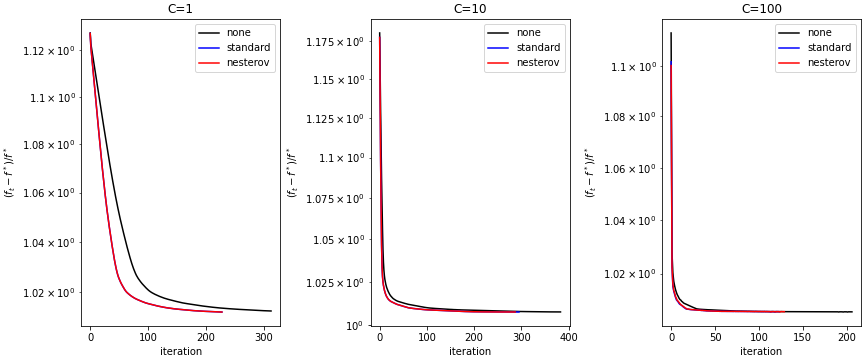
\includegraphics[scale=0.55]{img/l1_svc_loss_history}
	\caption{SGD Convergence for the Primal formulation of the $\protect \mathcal{L}_1$-SVC}
	\label{fig:l1_svc_history}
\end{figure}

\paragraph{Linear Dual formulations}

The experiments results shown in~\ref{linear_lagrangian_dual_l1_svc_cv_results} are obtained with $\alpha$, i.e., the \emph{learning rate} or \emph{step size}, setted to 0.001 for the \emph{AdaGrad} algorithm. Notice that the \emph{unreg\_bias} dual refers to the formulation~\eqref{eq:svc_lagrangian_dual}, while the \emph{reg\_bias} dual refers to the formulation~\eqref{eq:svc_bcqp_lagrangian_dual}.

\begin{table}[H]
\centering
\caption{Wolfe Dual linear $\protect \mathcal{L}_1$-SVC results}
\label{linear_dual_l1_svc_cv_results}
\begin{tabular}{llrrrr}
\toprule
       &     &  fit\_time &  accuracy &  n\_iter &  n\_sv \\
solver & C &           &           &         &       \\
\midrule
smo & 1   &  0.073731 &     0.980 &      62 &    17 \\
       & 10  &  0.146260 &     0.980 &     295 &    10 \\
       & 100 &  0.160641 &     0.985 &     399 &     8 \\
libsvm & 1   &  0.003538 &     0.985 &     243 &    17 \\
       & 10  &  0.002517 &     0.985 &     194 &    10 \\
       & 100 &  0.002370 &     0.985 &    1602 &     8 \\
cvxopt & 1   &  0.033754 &     0.980 &      10 &    17 \\
       & 10  &  0.026945 &     0.980 &      10 &    11 \\
       & 100 &  0.047614 &     0.980 &      10 &    12 \\
\bottomrule
\end{tabular}
\end{table}


For what about the linear \emph{Wolfe dual} formulation we can immediately notice as higher \emph{regularization hyperparameter} $C$ makes the model harder, so the \emph{custom} implementation of the SMO algorithm and also the \emph{sklearn} implementation, i.e., \emph{libsvm}~\cite{chang2011libsvm} implementation, needs to perform more iterations to achieve the same \emph{numerical precision}; meanwhile the \emph{cvxopt}~\cite{vandenberghe2010cvxopt} seems to be insensitive to the increasing complexity of the model. The results in terms of \emph{accuracy} and number of \emph{support vectors} are strongly similar to each others.

\begin{table}[H]
\centering
\caption{Lagrangian Dual linear $\protect \mathcal{L}_1$-SVC results}
\label{linear_lagrangian_dual_l1_svc_cv_results}
\begin{tabular}{llrrrr}
\toprule
           &     &  fit\_time &  accuracy &  n\_iter &  n\_sv \\
dual & C &           &           &         &       \\
\midrule
reg\_bias & 1   &  0.012731 &     0.985 &       1 &   194 \\
           & 10  &  0.019405 &     0.985 &       1 &   194 \\
           & 100 &  0.030348 &     0.985 &       1 &   194 \\
unreg\_bias & 1   &  0.034859 &     0.985 &       1 &   196 \\
           & 10  &  0.030251 &     0.985 &       1 &   196 \\
           & 100 &  0.031609 &     0.985 &       1 &   196 \\
\bottomrule
\end{tabular}
\end{table}


For what about the linear \emph{Lagrangian dual} formulation we can see as it seems to be insensitive to the increasing complexity of the model in terms of number of \emph{iterations} but it tends to select many training data points as \emph{support vectors}.

\paragraph{Nonlinear Dual formulations}

The experiments results shown in~\ref{nonlinear_dual_l1_svc_cv_results} and~\ref{nonlinear_lagrangian_dual_l1_svc_cv_results} are obtained with \emph{d} and \emph{r} hyperparameters equal to 3 and 1 respectively for the \emph{polynomial} kernel; \emph{gamma} is setted to \emph{`scale`} for both \emph{polynomial} and \emph{gaussian RBF} kernels. The experiments results shown in~\ref{nonlinear_lagrangian_dual_l1_svc_cv_results} are obtained with $\alpha$, i.e., the \emph{learning rate} or \emph{step size}, setted to 0.001 for the \emph{AdaGrad} algorithm.

\begin{table}[H]
\centering
\caption{Wolfe Dual nonlinear $\protect \mathcal{L}_1$-SVC results}
\label{nonlinear_dual_l1_svc_cv_results}
\begin{tabular}{lllrrrr}
\toprule
       &      &      &  fit\_time &  accuracy &  n\_iter &  n\_sv \\
solver & kernel & C &           &           &         &       \\
\midrule
smo & gaussian & 0.1  &  0.878962 &    1.0000 &      65 &   222 \\
       &      & 1.0  &  0.860773 &    1.0000 &      76 &    48 \\
       &      & 10.0 &  0.525582 &    1.0000 &      29 &    13 \\
       & poly & 0.1  &  1.096614 &    0.8675 &     121 &   142 \\
       &      & 1.0  &  0.999406 &    0.6825 &     143 &    30 \\
       &      & 10.0 &  0.680124 &    0.9475 &      65 &    10 \\
libsvm & gaussian & 0.1  &  0.011811 &    1.0000 &     131 &   222 \\
       &      & 1.0  &  0.007152 &    1.0000 &     252 &    50 \\
       &      & 10.0 &  0.003799 &    1.0000 &     134 &    13 \\
       & poly & 0.1  &  0.022929 &    1.0000 &     210 &   143 \\
       &      & 1.0  &  0.010823 &    1.0000 &     233 &    30 \\
       &      & 10.0 &  0.003304 &    1.0000 &     118 &    10 \\
cvxopt & gaussian & 0.1  &  0.426778 &    1.0000 &      10 &   222 \\
       &      & 1.0  &  0.568489 &    1.0000 &      10 &    49 \\
       &      & 10.0 &  0.557587 &    1.0000 &      10 &    14 \\
       & poly & 0.1  &  0.487677 &    0.8575 &      10 &   143 \\
       &      & 1.0  &  0.693849 &    0.6775 &      10 &    31 \\
       &      & 10.0 &  0.610578 &    0.9475 &      10 &    10 \\
\bottomrule
\end{tabular}
\end{table}


\begin{table}[H]
\centering
\caption{Lagrangian Dual nonlinear $\protect \mathcal{L}_1$-SVC results}
\label{nonlinear_lagrangian_dual_l1_svc_cv_results}
\begin{tabular}{lllrrrr}
\toprule
           &     &     &  fit\_time &  accuracy &  n\_iter &  n\_sv \\
dual & kernel & C &           &           &         &       \\
\midrule
reg\_bias & poly & 1   &  0.910125 &    0.6350 &     222 &   317 \\
           &     & 10  &  0.855964 &    0.6350 &     222 &   317 \\
           &     & 100 &  1.015074 &    0.6350 &     222 &   317 \\
           & rbf & 1   &  0.084307 &    1.0000 &       1 &   399 \\
           &     & 10  &  0.073900 &    1.0000 &       1 &   399 \\
           &     & 100 &  0.075157 &    1.0000 &       1 &   399 \\
unreg\_bias & poly & 1   &  0.069840 &    0.6075 &       3 &   314 \\
           &     & 10  &  0.068924 &    0.6075 &       3 &   314 \\
           &     & 100 &  0.058743 &    0.6075 &       3 &   314 \\
           & rbf & 1   &  0.117894 &    0.5000 &      11 &   115 \\
           &     & 10  &  0.359374 &    0.5575 &      46 &   282 \\
           &     & 100 &  0.385576 &    0.5575 &      46 &   282 \\
\bottomrule
\end{tabular}
\end{table}


The same considerations made for the previous linear \emph{Wolfe dual} and \emph{Lagrangian dual} formulations are confirmed also in the nonlinearly separable case. In this setting the complexity of the model coming with higher $C$ regularization values seems to be not paying a tradeoff in terms of the number of \emph{iterations} of the algorithm and, moreover, the \emph{reg\_bias Lagrangian dual} formulation seems to perform better wrt the \emph{unreg\_bias} formulation, both tends to select even more training data points as \emph{support vectors}.

\begin{figure}[H]
	\centering
	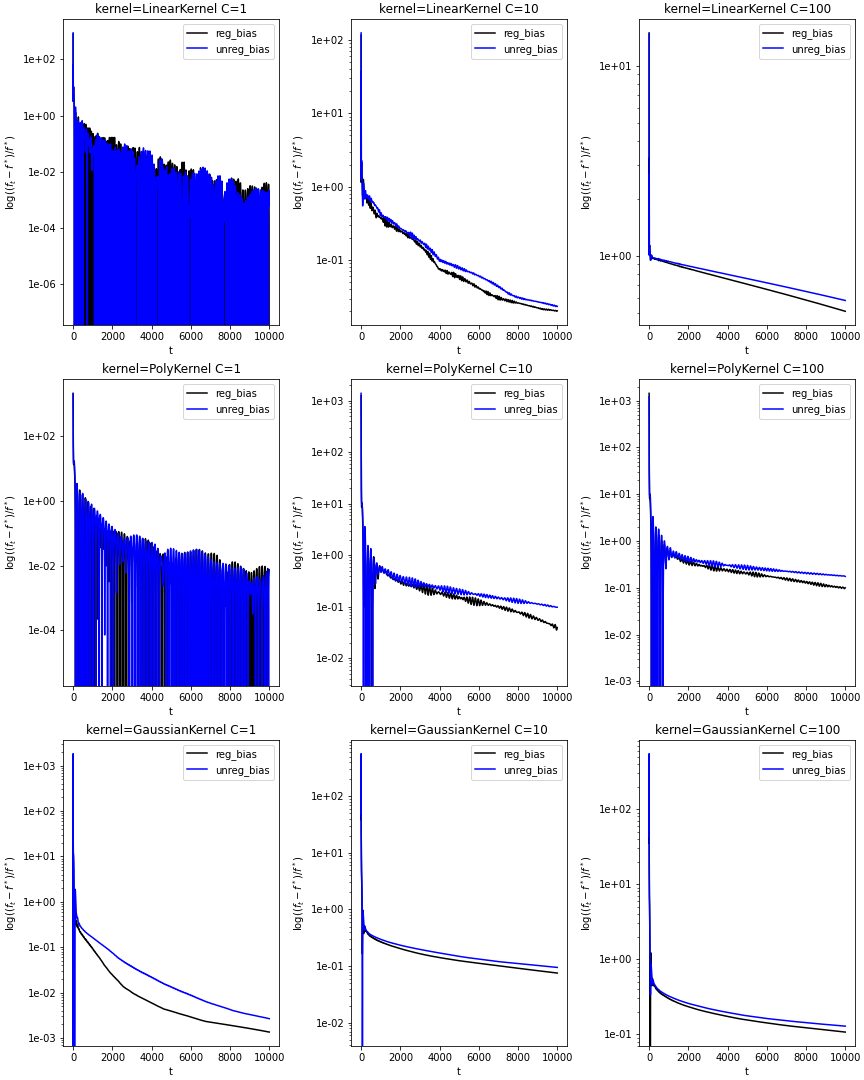
\includegraphics[scale=0.55]{img/lagrangian_dual_l1_svc_loss_history}
	\caption{AdaGrad convergence for the Lagrangian Dual formulation of the Nonlinear $\protect \mathcal{L}_1$-SVC}
	\label{fig:lagrangian_dual_l1_svc_loss_history}
\end{figure}

\pagebreak

\subsubsection{Squared Hinge loss}

\paragraph{Primal formulation}

The experiments results shown in~\ref{primal_l2_svc_cv_results} referred to \emph{Stochastic Gradient Descent} algorithm are obtained with $\alpha$, i.e., the \emph{learning rate} or \emph{step size}, setted to 0.001 and $\beta$, i.e., the \emph{momentum}, equal to 0.4. Training is stopped if after 5 iterations the training loss is not lower than the best found so far within a tolerance of $1\mathrm{e}{-8}$.

\begin{table}[H]
\centering
\caption{SVC Primal formulation results with Squared Hinge loss}
\label{primal_l2_svc_cv_results}
\begin{tabular}{lllrrrr}
\toprule
          &   &     &  fit\_time &  accuracy &  n\_iter &  n\_sv \\
solver & momentum & C &           &           &         &       \\
\midrule
sgd & none & 1   &  0.419254 &     0.975 &     154 &    49 \\
          &   & 10  &  0.314466 &     0.980 &     119 &    24 \\
          &   & 100 &  0.079897 &     0.985 &      30 &    15 \\
          & standard & 1   &  0.312977 &     0.975 &     113 &    45 \\
          &   & 10  &  0.203847 &     0.980 &      73 &    24 \\
          &   & 100 &  0.061971 &     0.985 &      21 &    11 \\
          & nesterov & 1   &  0.328923 &     0.970 &     132 &    40 \\
          &   & 10  &  0.188573 &     0.980 &      71 &    23 \\
          &   & 100 &  0.073157 &     0.985 &      26 &    10 \\
liblinear & - & 1   &  0.002038 &     0.980 &     556 &    25 \\
          &   & 10  &  0.002624 &     0.980 &    1000 &    19 \\
          &   & 100 &  0.002467 &     0.980 &    1000 &    27 \\
\bottomrule
\end{tabular}
\end{table}


Again, the results provided from the \emph{custom} implementation, i.e., the SGD with different momentum settings, are strongly similar to those of \emph{sklearn} implementation, i.e., \emph{liblinear}~\cite{fan2008liblinear} implementation, in terms of \emph{accuracy} score. More training data points are selected as \emph{support vectors} from the SGD solver but it always requires even lower iterations, i.e., epochs, to achieve the same \emph{numerical precision}. \emph{Standard} or \emph{Polyak} and \emph{Nesterov} momentums always perform lower iterations as expected from the theoretical analysis of the convergence rate.

\begin{figure}[H]
	\centering
	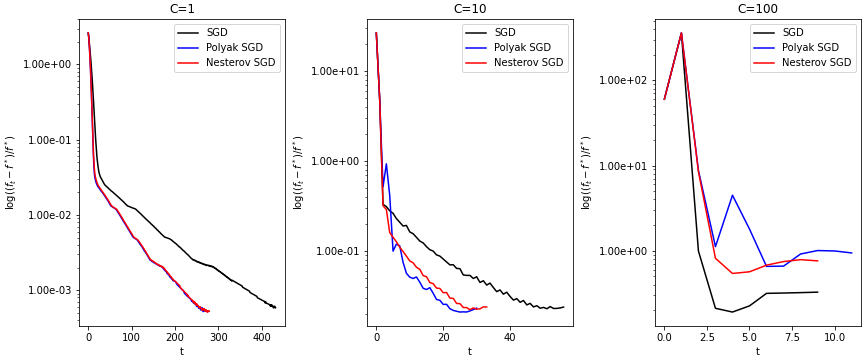
\includegraphics[scale=0.55]{img/l2_svc_loss_history}
	\caption{SGD convergence for the Primal formulation of the $\protect \mathcal{L}_2$-SVC}
	\label{fig:l2_svc_loss_history}
\end{figure}

\pagebreak

\subsection{Support Vector Regression}

Below experiments are about the SVR for which I tested different values for regularization hyperparameter $C$, i.e., from \emph{soft} to \emph{hard margin}, the $\epsilon$ penalty value and in case of nonlinearly separable data also different \emph{kernel functions} mentioned above.

The experiments about SVRs are available at: \\ \href{https://github.com/dmeoli/optiml/blob/master/notebooks/optimization/CM_SVR_report_experiments.ipynb}{\texttt{github.com/dmeoli/optiml/blob/master/notebooks/optimization/CM\_SVR\_report\_experiments.ipynb}}.

\subsubsection{Epsilon-insensitive loss}

\paragraph{Primal formulation}

The experiments results shown in~\ref{primal_l1_svr_cv_results} referred to \emph{Stochastic Gradient Descent} algorithm are obtained with $\alpha$, i.e., the \emph{learning rate} or \emph{step size}, setted to 0.001 and $\beta$, i.e., the \emph{momentum}, equal to 0.4. Training is stopped if after 5 iterations the training loss is not lower than the best found so far within a tolerance of $1\mathrm{e}{-8}$.

\begin{table}[H]
\centering
\caption{Primal $\protect \mathcal{L}_1$-SVR results}
\label{primal_l1_svr_cv_results}
\begin{tabular}{llllrrrr}
\toprule
          &   &     &     &   fit\_time &        r2 &  n\_iter &  n\_sv \\
solver & momentum & C & epsilon &            &           &         &       \\
\midrule
sgd & none & 1   & 0.1 &  13.207407 &  0.954298 &   16161 &   100 \\
          &   &     & 0.2 &   9.523358 &  0.954544 &   12267 &    99 \\
          &   &     & 0.3 &  11.594773 &  0.955424 &   13665 &    99 \\
          &   & 10  & 0.1 &   0.690761 &  0.983893 &     806 &    98 \\
          &   &     & 0.2 &   0.722907 &  0.983891 &     884 &    98 \\
          &   &     & 0.3 &   0.756686 &  0.983884 &     958 &    97 \\
          &   & 100 & 0.1 &   0.121053 &  0.984034 &      85 &    97 \\
          &   &     & 0.2 &   0.088140 &  0.984047 &      96 &    98 \\
          &   &     & 0.3 &   0.156799 &  0.984056 &     109 &    98 \\
          & polyak & 1   & 0.1 &   7.895537 &  0.954321 &    9874 &   100 \\
          &   &     & 0.2 &   5.816864 &  0.954549 &    7400 &    99 \\
          &   &     & 0.3 &   6.935173 &  0.955424 &    8200 &    99 \\
          &   & 10  & 0.1 &   0.489926 &  0.983893 &     487 &    97 \\
          &   &     & 0.2 &   0.503936 &  0.983891 &     535 &    98 \\
          &   &     & 0.3 &   0.483785 &  0.983885 &     569 &    98 \\
          &   & 100 & 0.1 &   0.090085 &  0.984030 &      48 &    98 \\
          &   &     & 0.2 &   0.108489 &  0.984046 &      56 &    98 \\
          &   &     & 0.3 &   0.114756 &  0.984055 &      61 &    97 \\
          & nesterov & 1   & 0.1 &   8.996545 &  0.954310 &    9785 &   100 \\
          &   &     & 0.2 &   6.001156 &  0.954546 &    7382 &    99 \\
          &   &     & 0.3 &   7.318327 &  0.955424 &    8198 &    99 \\
          &   & 10  & 0.1 &   0.803194 &  0.983892 &     489 &    97 \\
          &   &     & 0.2 &   0.457146 &  0.983890 &     533 &    97 \\
          &   &     & 0.3 &   0.561535 &  0.983884 &     579 &    98 \\
          &   & 100 & 0.1 &   0.097744 &  0.984031 &      61 &    98 \\
          &   &     & 0.2 &   0.120314 &  0.984047 &      58 &    98 \\
          &   &     & 0.3 &   0.107943 &  0.984057 &      62 &    98 \\
liblinear & - & 1   & 0.1 &   0.019717 &  0.954684 &      12 &   100 \\
          &   &     & 0.2 &   0.001534 &  0.955112 &      10 &    99 \\
          &   &     & 0.3 &   0.001302 &  0.955415 &      10 &    97 \\
          &   & 10  & 0.1 &   0.002194 &  0.983893 &      57 &    99 \\
          &   &     & 0.2 &   0.001483 &  0.983890 &      69 &    98 \\
          &   &     & 0.3 &   0.001968 &  0.983906 &     142 &    97 \\
          &   & 100 & 0.1 &   0.001972 &  0.984023 &     980 &    97 \\
          &   &     & 0.2 &   0.006431 &  0.984028 &    1340 &    97 \\
          &   &     & 0.3 &   0.002328 &  0.984051 &    2886 &    97 \\
\bottomrule
\end{tabular}
\end{table}


The results provided from the \emph{custom} implementation, i.e., the SGD with different momentum settings, are strongly similar to those of \emph{sklearn} implementation, i.e., \emph{liblinear}~\cite{fan2008liblinear} implementation, in terms of \emph{r2} score, except in case of $C$ regularization hyperparameter equals to 1 for which those of SGD are lower. Moreover, the SGD solver always requires lower iterations, i.e., epochs, for higher $C$ regularization values, i.e., for $C$ equals to 10 or 100, to achieve the same \emph{numerical precision}. Again, \emph{Standard} or \emph{Polyak} and \emph{Nesterov} momentums always perform lower iterations as expected from the theoretical analysis of the convergence rate. The results in terms of \emph{support vectors} are strongly similar to each others.

\begin{figure}[H]
	\centering
	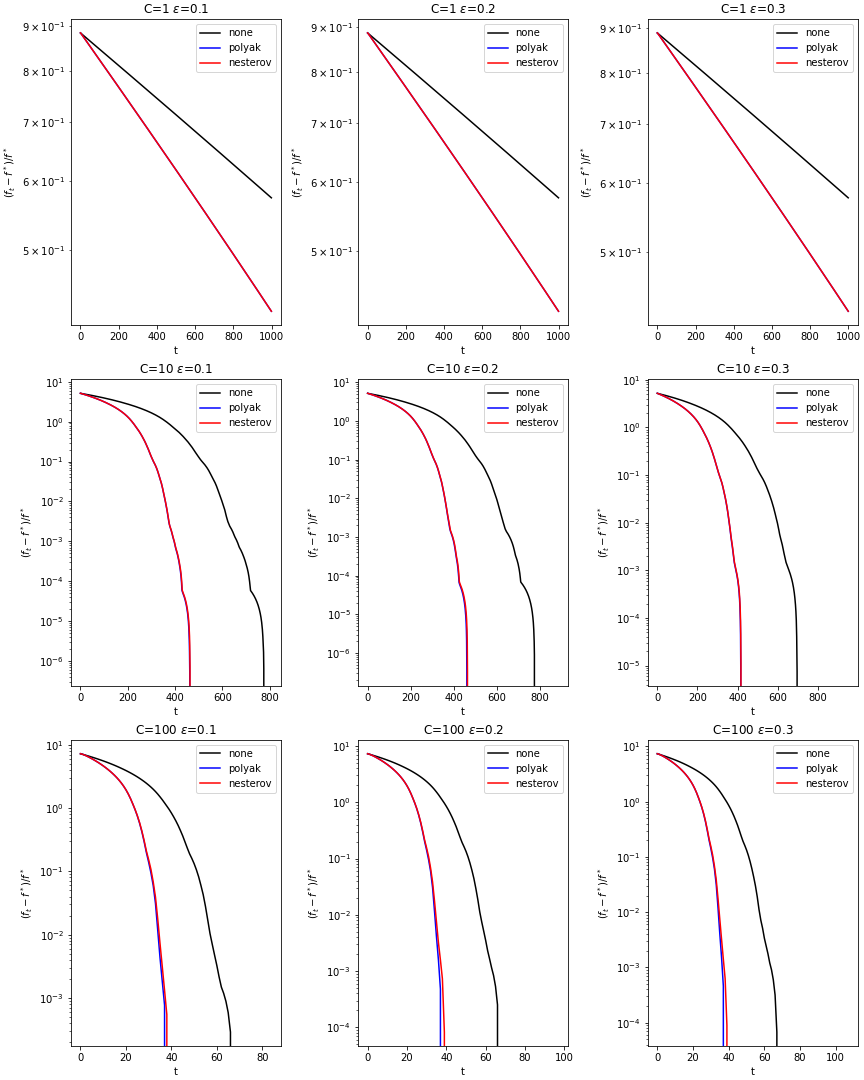
\includegraphics[scale=0.5]{img/l1_svr_loss_history}
	\caption{SGD convergence for the Primal formulation of the $\protect \mathcal{L}_1$-SVR}
	\label{fig:l1_svr_loss_history}
\end{figure}

\pagebreak

\paragraph{Linear Dual formulations}

The experiments results shown in~\ref{linear_lagrangian_dual_l1_svr_cv_results} are obtained with $\alpha$, i.e., the \emph{learning rate} or \emph{step size}, setted to 0.001 for the \emph{AdaGrad} algorithm. Notice that the \emph{unreg\_bias} dual refers to the formulation~\eqref{eq:svr_lagrangian_dual}, while the \emph{reg\_bias} dual refers to the formulation~\eqref{eq:svr_bcqp_lagrangian_dual}.

\begin{table}[H]
\centering
\caption{Wolfe Dual linear $\protect \mathcal{L}_1$-SVR results}
\label{linear_dual_l1_svr_cv_results}
\begin{tabular}{lllrrrr}
\toprule
       &     &     &  fit\_time &        r2 &  n\_iter &  n\_sv \\
solver & C & epsilon &           &           &         &       \\
\midrule
smo & 1   & 0.1 &  0.049352 &  0.954396 &      10 &   100 \\
       &     & 0.2 &  0.026155 &  0.954546 &      15 &   100 \\
       &     & 0.3 &  0.090050 &  0.955429 &      13 &    99 \\
       & 10  & 0.1 &  0.201986 &  0.983893 &      44 &    99 \\
       &     & 0.2 &  0.091500 &  0.983893 &      48 &    99 \\
       &     & 0.3 &  0.084329 &  0.983893 &      41 &    99 \\
       & 100 & 0.1 &  0.826075 &  0.984071 &     623 &    98 \\
       &     & 0.2 &  0.409304 &  0.984088 &     157 &    98 \\
       &     & 0.3 &  0.521488 &  0.984103 &     334 &    98 \\
libsvm & 1   & 0.1 &  0.009594 &  0.954393 &      79 &   100 \\
       &     & 0.2 &  0.005095 &  0.954543 &      82 &   100 \\
       &     & 0.3 &  0.029558 &  0.955424 &      78 &    99 \\
       & 10  & 0.1 &  0.033350 &  0.983892 &     206 &    99 \\
       &     & 0.2 &  0.005173 &  0.983890 &     219 &    99 \\
       &     & 0.3 &  0.009250 &  0.983885 &     216 &    99 \\
       & 100 & 0.1 &  0.019970 &  0.984028 &    2239 &    98 \\
       &     & 0.2 &  0.006288 &  0.984041 &    1189 &    98 \\
       &     & 0.3 &  0.003961 &  0.984051 &    1366 &    98 \\
cvxopt & 1   & 0.1 &  0.122198 &  0.954685 &       9 &   100 \\
       &     & 0.2 &  0.152970 &  0.954849 &       9 &   100 \\
       &     & 0.3 &  0.066905 &  0.955429 &      10 &   100 \\
       & 10  & 0.1 &  0.144911 &  0.983893 &       9 &   100 \\
       &     & 0.2 &  0.056698 &  0.983893 &       8 &   100 \\
       &     & 0.3 &  0.045109 &  0.983893 &       8 &   100 \\
       & 100 & 0.1 &  0.094987 &  0.984071 &       9 &   100 \\
       &     & 0.2 &  0.070957 &  0.984088 &       9 &   100 \\
       &     & 0.3 &  0.095619 &  0.984103 &       8 &   100 \\
\bottomrule
\end{tabular}
\end{table}


For what about the linear \emph{Wolfe dual} formulation we can immediately notice as higher \emph{regularization hyperparameter} $C$ and lower $\epsilon$ values makes the model harder, so the \emph{custom} implementation of the SMO algorithm and also the \emph{sklearn} implementation, i.e., \emph{libsvm}~\cite{chang2011libsvm} implementation, needs to perform more iterations to achieve the same \emph{numerical precision}; meanwhile, again, the \emph{cvxopt}~\cite{vandenberghe2010cvxopt} seems to be insensitive to the increasing complexity of the model. The results in terms of \emph{r2} and number of \emph{support vectors} are strongly similar to each others.

\begin{table}[H]
\centering
\caption{Lagrangian Dual linear $\protect \mathcal{L}_1$-SVR results}
\label{linear_lagrangian_dual_l1_svr_cv_results}
\begin{tabular}{lllrrrr}
\toprule
           &     &     &    fit\_time &        r2 &  n\_iter &  n\_sv \\
dual & C & epsilon &             &           &         &       \\
\midrule
reg\_bias & 1   & 0.1 &   23.881113 &  0.954685 &   22445 &   100 \\
           &     & 0.2 &   31.481934 &  0.954845 &   22235 &   100 \\
           &     & 0.3 &   24.310760 &  0.955429 &   21493 &    99 \\
           & 10  & 0.1 &   43.878878 &  0.983893 &   24700 &    99 \\
           &     & 0.2 &   43.092336 &  0.983893 &   26586 &    99 \\
           &     & 0.3 &   60.609057 &  0.983893 &   26076 &    99 \\
           & 100 & 0.1 &  151.873868 &  0.984071 &  105273 &    98 \\
           &     & 0.2 &  173.833673 &  0.984088 &  141626 &    98 \\
           &     & 0.3 &  259.661015 &  0.984103 &  284365 &    98 \\
unreg\_bias & 1   & 0.1 &   49.656317 &  0.954396 &   24597 &   100 \\
           &     & 0.2 &   83.297098 &  0.954546 &   62678 &   100 \\
           &     & 0.3 &  313.268643 &  0.955429 &  332397 &    99 \\
           & 10  & 0.1 &   67.435317 &  0.983893 &   55824 &    99 \\
           &     & 0.2 &   85.381756 &  0.983893 &   56708 &    99 \\
           &     & 0.3 &  100.468285 &  0.983893 &   62786 &    99 \\
           & 100 & 0.1 &  675.775826 &  0.984071 &  491963 &    98 \\
           &     & 0.2 &  636.590656 &  0.984088 &  541088 &    98 \\
           &     & 0.3 &  634.562593 &  0.984103 &  674048 &    98 \\
\bottomrule
\end{tabular}
\end{table}


For what about the linear \emph{Lagrangian dual} formulation we can see as it seems to be insensitive to the increasing complexity of the model in terms of number of \emph{iterations} and require many \emph{iterations} wrt the \emph{Wolfe dual} formulation.

\begin{figure}[H]
	\centering
	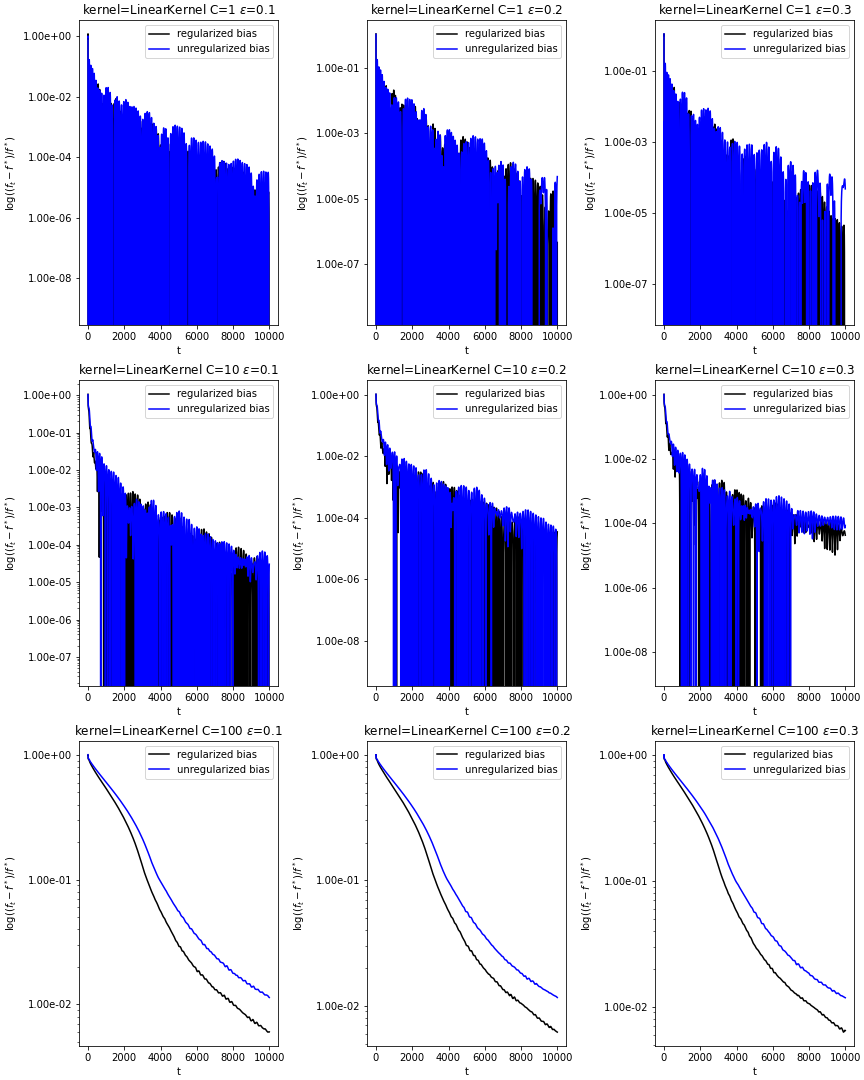
\includegraphics[scale=0.55]{img/linear_lagrangian_dual_l1_svr_loss_history}
	\caption{AdaGrad convergence for the Lagrangian Dual formulation of the Linear $\protect \mathcal{L}_1$-SVR}
	\label{fig:linear_lagrangian_dual_l1_svr_loss_history}
\end{figure}

\paragraph{Nonlinear Dual formulations}

The experiments results shown in~\ref{nonlinear_dual_l1_svr_cv_results} and~\ref{nonlinear_lagrangian_dual_l1_svr_cv_results} are obtained with \emph{d} and \emph{r} hyperparameters both equal to 3 for the \emph{polynomial} kernel; \emph{gamma} is setted to \emph{`scale`} for both \emph{polynomial} and \emph{gaussian RBF} kernels. The experiments results shown in~\ref{nonlinear_lagrangian_dual_l1_svc_cv_results} are obtained with $\alpha$, i.e., the \emph{learning rate} or \emph{step size}, setted to 0.001 for the \emph{AdaGrad} algorithm.

\begin{table}[H]
\centering
\caption{Wolfe Dual nonlinear $\protect \mathcal{L}_1$-SVR formulation results}
\label{nonlinear_dual_l1_svr_cv_results}
\begin{tabular}{llllrrrr}
\toprule
       &     &     &     &     fit\_time &        r2 &    n\_iter &  n\_sv \\
solver & kernel & C & epsilon &              &           &           &       \\
\midrule
smo & poly & 1   & 0.1 &    71.647312 &  0.810056 &     47694 &    36 \\
       &     &     & 0.2 &    12.618369 &  0.671256 &      8702 &     6 \\
       &     &     & 0.3 &     4.557922 &  0.302709 &      3654 &     4 \\
       &     & 10  & 0.1 &   318.425233 &  0.736098 &    256531 &    32 \\
       &     &     & 0.2 &    39.047974 &  0.923152 &     32629 &     4 \\
       &     &     & 0.3 &     4.677411 &  0.302709 &      3654 &     4 \\
       &     & 100 & 0.1 &  2086.026956 &  0.635585 &   3294613 &    33 \\
       &     &     & 0.2 &    40.670991 &  0.923152 &     32629 &     4 \\
       &     &     & 0.3 &     4.617724 &  0.302709 &      3654 &     4 \\
       & rbf & 1   & 0.1 &     0.054718 &  0.988244 &        66 &    17 \\
       &     &     & 0.2 &     0.018531 &  0.924292 &        20 &     7 \\
       &     &     & 0.3 &     0.016346 &  0.883022 &        17 &     5 \\
       &     & 10  & 0.1 &     0.440781 &  0.989739 &       389 &    18 \\
       &     &     & 0.2 &     0.027589 &  0.924995 &        25 &     6 \\
       &     &     & 0.3 &     0.007014 &  0.882816 &        11 &     5 \\
       &     & 100 & 0.1 &     3.799744 &  0.974756 &      6664 &    19 \\
       &     &     & 0.2 &     0.024482 &  0.924995 &        25 &     6 \\
       &     &     & 0.3 &     0.011137 &  0.882816 &        11 &     5 \\
libsvm & poly & 1   & 0.1 &     0.049065 &  0.981438 &    155092 &    37 \\
       &     &     & 0.2 &     0.015740 &  0.976358 &      7326 &     6 \\
       &     &     & 0.3 &     0.004452 &  0.951282 &      3969 &     4 \\
       &     & 10  & 0.1 &     0.166962 &  0.981769 &    578347 &    32 \\
       &     &     & 0.2 &     0.019647 &  0.979414 &     28452 &     4 \\
       &     &     & 0.3 &     0.004198 &  0.951282 &      3969 &     4 \\
       &     & 100 & 0.1 &     2.349179 &  0.981844 &  13306191 &    35 \\
       &     &     & 0.2 &     0.009665 &  0.979414 &     28452 &     4 \\
       &     &     & 0.3 &     0.012851 &  0.951282 &      3969 &     4 \\
       & rbf & 1   & 0.1 &     0.005776 &  0.990088 &        96 &    17 \\
       &     &     & 0.2 &     0.020616 &  0.977763 &        36 &     7 \\
       &     &     & 0.3 &     0.001456 &  0.945601 &        24 &     5 \\
       &     & 10  & 0.1 &     0.002339 &  0.990493 &       616 &    18 \\
       &     &     & 0.2 &     0.010448 &  0.980673 &        39 &     6 \\
       &     &     & 0.3 &     0.007578 &  0.945601 &        24 &     5 \\
       &     & 100 & 0.1 &     0.005937 &  0.990496 &      9854 &    18 \\
       &     &     & 0.2 &     0.008988 &  0.980673 &        39 &     6 \\
       &     &     & 0.3 &     0.002329 &  0.945601 &        24 &     5 \\
cvxopt & poly & 1   & 0.1 &     0.065255 &  0.828482 &        10 &    37 \\
       &     &     & 0.2 &     0.041122 &  0.666571 &        10 &     6 \\
       &     &     & 0.3 &     0.029873 &  0.350876 &         9 &     4 \\
       &     & 10  & 0.1 &     0.048030 &  0.629433 &        10 &    33 \\
       &     &     & 0.2 &     0.064068 &  0.928477 &        10 &     4 \\
       &     &     & 0.3 &     0.063453 &  0.350873 &        10 &     4 \\
       &     & 100 & 0.1 &     0.063773 &  0.712681 &        10 &    36 \\
       &     &     & 0.2 &     0.097430 &  0.928478 &        10 &     4 \\
       &     &     & 0.3 &     0.072250 &  0.350876 &        10 &     4 \\
       & rbf & 1   & 0.1 &     0.039900 &  0.988117 &        10 &    17 \\
       &     &     & 0.2 &     0.030282 &  0.924679 &        10 &     7 \\
       &     &     & 0.3 &     0.047886 &  0.883386 &        10 &     5 \\
       &     & 10  & 0.1 &     0.022933 &  0.989956 &        10 &    18 \\
       &     &     & 0.2 &     0.022819 &  0.925595 &        10 &     6 \\
       &     &     & 0.3 &     0.032468 &  0.883386 &        10 &     5 \\
       &     & 100 & 0.1 &     0.022127 &  0.990216 &        10 &    40 \\
       &     &     & 0.2 &     0.037909 &  0.925595 &        10 &     6 \\
       &     &     & 0.3 &     0.029582 &  0.883386 &        10 &     5 \\
\bottomrule
\end{tabular}
\end{table}


\begin{table}[H]
\centering
\caption{Lagrangian Dual nonlinear $\protect \mathcal{L}_1$-SVR results}
\label{nonlinear_lagrangian_dual_l1_svr_cv_results}
\begin{tabular}{llllrrrr}
\toprule
           &     &     &     &   fit\_time &        r2 &  n\_iter &  n\_sv \\
dual & kernel & C & epsilon &            &           &         &       \\
\midrule
reg\_bias & poly & 1   & 0.1 &   9.014323 &  0.980130 &   10000 &   100 \\
           &     &     & 0.2 &   7.949212 &  0.978522 &   10000 &   100 \\
           &     &     & 0.3 &   8.145561 &  0.975487 &   10000 &    99 \\
           &     & 10  & 0.1 &   8.056295 &  0.975741 &   10000 &   100 \\
           &     &     & 0.2 &   7.586514 &  0.965786 &   10000 &   100 \\
           &     &     & 0.3 &   7.546005 &  0.954454 &   10000 &   100 \\
           &     & 100 & 0.1 &   8.766536 &  0.975741 &   10000 &   100 \\
           &     &     & 0.2 &   7.580433 &  0.965786 &   10000 &   100 \\
           &     &     & 0.3 &   7.518447 &  0.954454 &   10000 &   100 \\
           & rbf & 1   & 0.1 &   9.239836 &  0.983938 &   10000 &    49 \\
           &     &     & 0.2 &   9.088686 &  0.977767 &   10000 &    17 \\
           &     &     & 0.3 &   9.433860 &  0.944901 &   10000 &    58 \\
           &     & 10  & 0.1 &   9.681272 &  0.988661 &   10000 &    37 \\
           &     &     & 0.2 &   8.926462 &  0.985573 &   10000 &    38 \\
           &     &     & 0.3 &   9.579983 &  0.938212 &   10000 &    37 \\
           &     & 100 & 0.1 &   9.050977 &  0.988661 &   10000 &    37 \\
           &     &     & 0.2 &   9.211919 &  0.985573 &   10000 &    38 \\
           &     &     & 0.3 &  10.618364 &  0.938212 &   10000 &    37 \\
unreg\_bias & poly & 1   & 0.1 &   8.242731 &  0.980066 &   10000 &   100 \\
           &     &     & 0.2 &   7.870472 &  0.977327 &   10000 &   100 \\
           &     &     & 0.3 &   7.946662 &  0.976209 &   10000 &   100 \\
           &     & 10  & 0.1 &   7.509824 &  0.976242 &   10000 &   100 \\
           &     &     & 0.2 &   7.686515 &  0.969756 &   10000 &   100 \\
           &     &     & 0.3 &   7.510774 &  0.952895 &   10000 &   100 \\
           &     & 100 & 0.1 &   7.761488 &  0.976242 &   10000 &   100 \\
           &     &     & 0.2 &   7.630195 &  0.969756 &   10000 &   100 \\
           &     &     & 0.3 &   7.696242 &  0.952895 &   10000 &   100 \\
           & rbf & 1   & 0.1 &   9.121422 &  0.989997 &   10000 &    98 \\
           &     &     & 0.2 &   9.455734 &  0.977496 &   10000 &    57 \\
           &     &     & 0.3 &   9.615668 &  0.938677 &   10000 &    85 \\
           &     & 10  & 0.1 &   9.210732 &  0.989394 &   10000 &    83 \\
           &     &     & 0.2 &   9.280972 &  0.977514 &   10000 &    53 \\
           &     &     & 0.3 &   9.276510 &  0.939582 &   10000 &    67 \\
           &     & 100 & 0.1 &   8.975165 &  0.989394 &   10000 &    83 \\
           &     &     & 0.2 &   9.288849 &  0.977514 &   10000 &    53 \\
           &     &     & 0.3 &   8.827427 &  0.939582 &   10000 &    67 \\
\bottomrule
\end{tabular}
\end{table}


The same considerations made for the previous linear \emph{Wolfe dual} and \emph{Lagrangian dual} formulations are confirmed also in the nonlinearly separable case. In this setting, the complexity of the model coming with higher $C$ regularization hyperparameters and lower $\epsilon$ values pays a larger tradeoff in terms of the number of \emph{iterations} of the algorithm.

\begin{figure}[H]
	\centering
	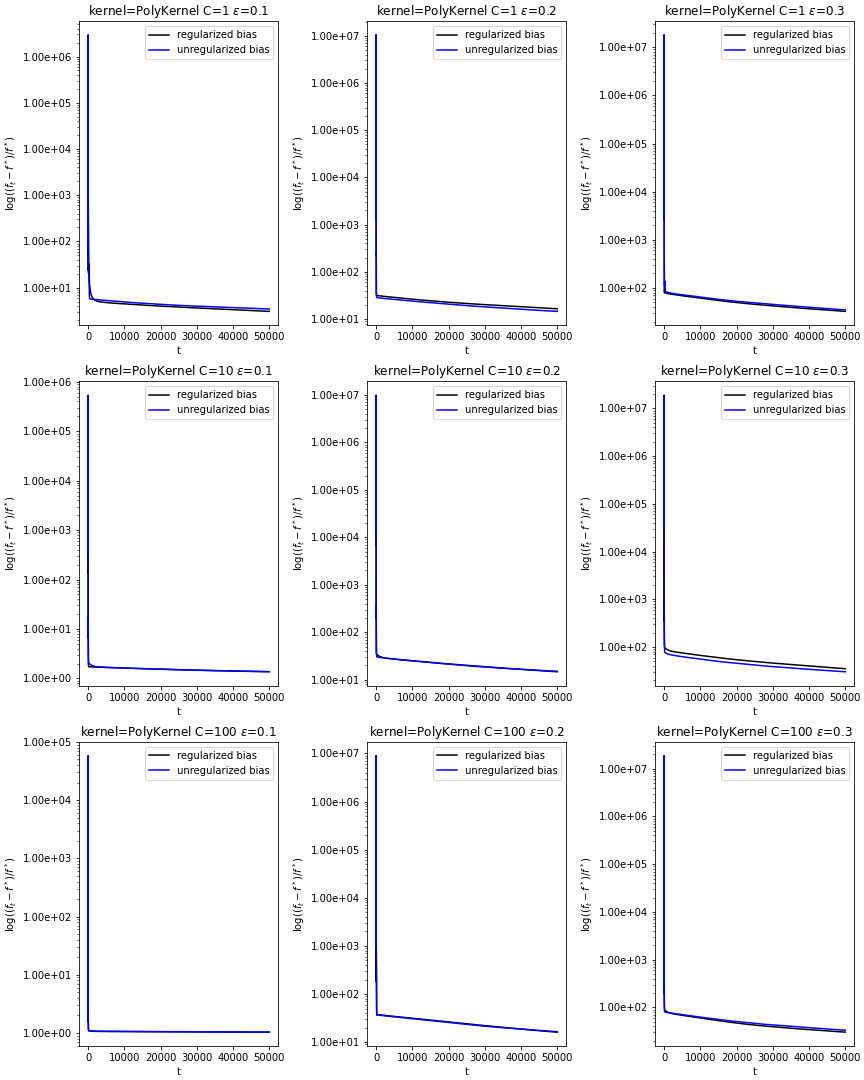
\includegraphics[scale=0.55]{img/poly_lagrangian_dual_l1_svr_loss_history}
	\caption{AdaGrad convergence for the Lagrangian Dual formulation of the Polynomial $\protect \mathcal{L}_1$-SVR}
	\label{fig:poly_lagrangian_dual_l1_svr_loss_history}
\end{figure}

\begin{figure}[H]
	\centering
	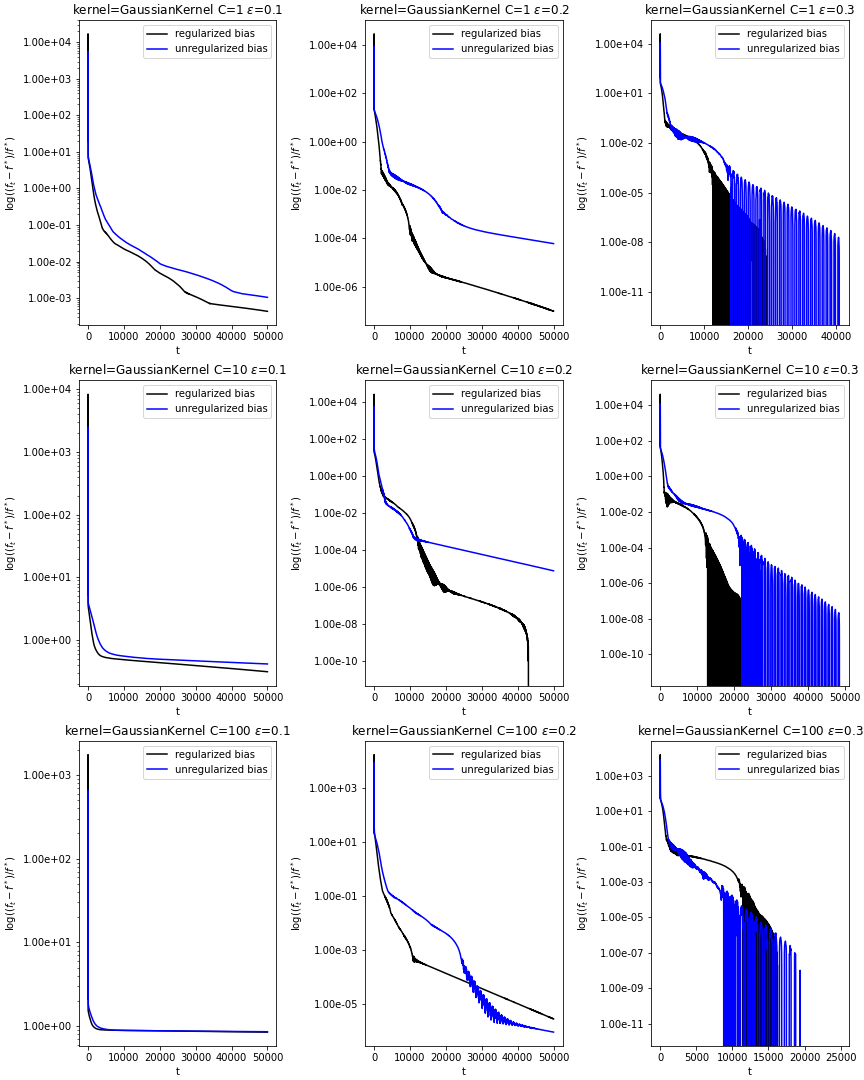
\includegraphics[scale=0.55]{img/gaussian_lagrangian_dual_l1_svr_loss_history}
	\caption{AdaGrad convergence for the Lagrangian Dual formulation of the Gaussian $\protect \mathcal{L}_1$-SVR}
	\label{fig:gaussian_lagrangian_dual_l1_svr_loss_history}
\end{figure}

\pagebreak

\subsubsection{Squared Epsilon-insensitive loss}

\paragraph{Primal formulation}

The experiments results shown in~\ref{primal_l2_svr_cv_results} referred to \emph{Stochastic Gradient Descent} algorithm are obtained with $\alpha$, i.e., the \emph{learning rate} or \emph{step size}, setted to 0.001 and $\beta$, i.e., the \emph{momentum}, equal to 0.4. Training is stopped if after 5 iterations the training loss is not lower than the best found so far within a tolerance of $1\mathrm{e}{-8}$.

\begin{table}[H]
\centering
\caption{Primal $\protect \mathcal{L}_2$-SVR results}
\label{primal_l2_svr_cv_results}
\begin{tabular}{llllrrrr}
\toprule
          &   &     &     &  fit\_time &        r2 &  n\_iter &  n\_sv \\
solver & momentum & C & epsilon &           &           &         &       \\
\midrule
sgd & none & 1   & 0.1 &  0.628824 &  0.977019 &     652 &   100 \\
          &   &     & 0.2 &  0.604419 &  0.977008 &     655 &    99 \\
          &   &     & 0.3 &  0.594717 &  0.976996 &     657 &    99 \\
          &   & 10  & 0.1 &  0.069660 &  0.977572 &      75 &    99 \\
          &   &     & 0.2 &  0.069005 &  0.977572 &      75 &    99 \\
          &   &     & 0.3 &  0.070856 &  0.977571 &      76 &    99 \\
          &   & 100 & 0.1 &  0.008819 &  0.977413 &       8 &   100 \\
          &   &     & 0.2 &  0.009804 &  0.977418 &       9 &    99 \\
          &   &     & 0.3 &  0.009794 &  0.977423 &       9 &    98 \\
          & standard & 1   & 0.1 &  0.397914 &  0.977028 &     405 &   100 \\
          &   &     & 0.2 &  0.371360 &  0.977018 &     407 &    99 \\
          &   &     & 0.3 &  0.379346 &  0.977006 &     408 &    99 \\
          &   & 10  & 0.1 &  0.040419 &  0.977572 &      42 &    99 \\
          &   &     & 0.2 &  0.043567 &  0.977571 &      42 &    99 \\
          &   &     & 0.3 &  0.041749 &  0.977571 &      43 &    99 \\
          &   & 100 & 0.1 &  0.007162 &  0.977443 &       6 &    99 \\
          &   &     & 0.2 &  0.006814 &  0.977447 &       6 &    99 \\
          &   &     & 0.3 &  0.007255 &  0.977450 &       6 &    97 \\
          & nesterov & 1   & 0.1 &  0.403233 &  0.977028 &     406 &   100 \\
          &   &     & 0.2 &  0.376248 &  0.977018 &     408 &    99 \\
          &   &     & 0.3 &  0.379239 &  0.977006 &     409 &    99 \\
          &   & 10  & 0.1 &  0.040307 &  0.977572 &      43 &    99 \\
          &   &     & 0.2 &  0.043603 &  0.977571 &      43 &    99 \\
          &   &     & 0.3 &  0.041826 &  0.977570 &      43 &    99 \\
          &   & 100 & 0.1 &  0.007321 &  0.977417 &       6 &   100 \\
          &   &     & 0.2 &  0.007085 &  0.977423 &       6 &    99 \\
          &   &     & 0.3 &  0.007221 &  0.977428 &       6 &    98 \\
liblinear & - & 1   & 0.1 &  0.000905 &  0.977554 &      96 &   100 \\
          &   &     & 0.2 &  0.001104 &  0.977553 &      96 &   100 \\
          &   &     & 0.3 &  0.001333 &  0.977551 &      96 &   100 \\
          &   & 10  & 0.1 &  0.003077 &  0.977577 &     826 &   100 \\
          &   &     & 0.2 &  0.003161 &  0.977576 &     826 &    99 \\
          &   &     & 0.3 &  0.003165 &  0.977576 &     839 &    99 \\
          &   & 100 & 0.1 &  0.003899 &  0.977538 &    1000 &   100 \\
          &   &     & 0.2 &  0.003790 &  0.977540 &    1000 &    99 \\
          &   &     & 0.3 &  0.004260 &  0.977541 &    1000 &    98 \\
\bottomrule
\end{tabular}
\end{table}


Again, the results provided from the \emph{custom} implementation, i.e., the SGD with different momentum settings, are strongly similar to those of \emph{sklearn} implementation, i.e., \emph{liblinear}~\cite{fan2008liblinear} implementation, in terms of \emph{r2} score. SGD solver always requires even lower iterations, i.e., epochs, for higher $C$ regularization values, i.e., for $C$ equals to 10 or 100, to achieve the same \emph{numerical precision}. \emph{Standard} or \emph{Polyak} and \emph{Nesterov} momentums always perform lower iterations as expected from the theoretical analysis of the convergence rate.

\begin{figure}[H]
	\centering
	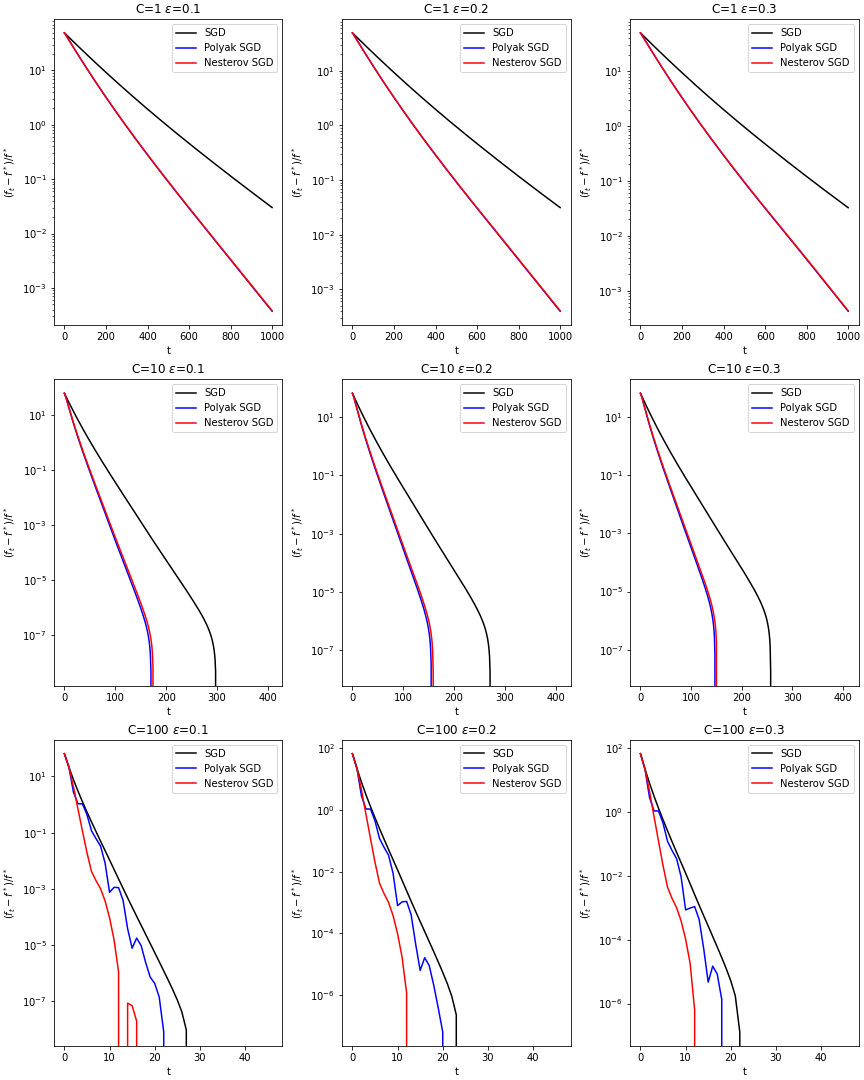
\includegraphics[scale=0.5]{img/l2_svr_loss_history}
	\caption{SGD convergence for the Primal formulation of the $\protect \mathcal{L}_2$-SVR}
	\label{fig:l2_svr_loss_history}
\end{figure}
